\section{Bounding Dirichlet series}

In view of Corollary \ref{zero-test}, it is of interest to obtain lower bounds for the quantity $f_t(x+iy)$ defined in \eqref{ft-def}
for $x,y,t$ in the region \eqref{region}.  By the triangle inequality (and the trivial identity $|z| = |\overline{z}|$), we obtain the lower bound
$$ |f_t(x+iy)| \geq \left( \left| \sum_{n=1}^N \frac{b_n^t}{n^{s_*}}\right| - |\gamma| \left| \sum_{n=1}^N n^y \frac{b_n^t}{n^{s_* + \overline{\kappa}}} \right|\right)_+.$$

It is thus of interest to obtain lower bounds for differences
\begin{equation}\label{Delta-def}
 \Delta \coloneqq \left( \left| \sum_{n=1}^N \frac{\beta_n}{n^s}\right| - \left| \sum_{n=1}^N \frac{\alpha_n}{n^s}\right| \right)_+
\end{equation}
of magnitudes of Dirichlet series for various coefficients $\beta_n, \alpha_n$.  Our tools for this will be as follows.

\begin{lemma}\label{dirb}  Let $N$ be a natural number, let $s = \sigma+iT$ be a complex number for some real $\sigma,T$, and let $\alpha_n,\beta_n$ be complex numbers for $n=1,\dots,N$ with $\beta_1=1$.  Let $\Delta$ denote the quantity \eqref{Delta-def}.
\begin{itemize}
\item[(i)]  (Triangle inequality) We have
$$ \Delta \geq 1 - \alpha_1 - \sum_{n=2}^N \frac{|\alpha_n| + |\beta_n|}{n^\sigma}.$$
\item[(ii)]  (Refined triangle inequality) If the $\alpha_n,\beta_n$ are all real and $0 \leq \alpha_1 <1$, then we have 
$$ \Delta \geq 1 - \alpha_1 - \sum_{n=2}^N \frac{\max( |\beta_n-\alpha_n|, \frac{1-\alpha_1}{1+\alpha_1} |\beta_n+\alpha_n|)}{n^\sigma}.$$
\item[(iii)]  (Dirichlet mollifier)  If $\lambda_1,\dots,\lambda_D$ are complex numbers, not all zero, then
$$ \Delta \geq \frac{\tilde \Delta}{\sum_{d=1}^D \frac{|\lambda_d|}{d^\sigma}} $$
where
$$ \tilde \Delta \coloneqq \left( \left| \sum_{n=1}^{DN} \frac{\tilde \beta_n}{n^s}\right| - \left| \sum_{n=1}^{DN} \frac{\tilde \alpha_n}{n^s}\right| \right)_+$$
and $\tilde \alpha_n, \tilde \beta_n$ are the Dirichlet convolutions of $\alpha_n,\beta_n$ with the $\lambda_d$:
\begin{align*}
\tilde \alpha_n &\coloneqq \sum_{1 \leq d \leq D: d|n} \lambda_d \alpha_{n/d} \\
\tilde \beta_n &\coloneqq \sum_{1 \leq d \leq D: d|n} \lambda_d \beta_{n/d}.
\end{align*}
\end{itemize}
\end{lemma}

\begin{proof}  The claim (i) is immediate from the triangle inequality.

Now we prove (ii).  We may assume that the right-hand side is positive, as the claim is trivial otherwise.  By a continuity argument (replacing $\beta_n,\alpha_n$ for $n \geq 2$ by $t \beta_n, t \alpha_n$ with $t$ increasing continuously from zero to one, noting that this only increases the right-hand side of the inequality) it suffices to verify the claim when $\Delta$ is positive.  In this case, we may write
$$ \Delta = \left|\sum_{n=1}^N \frac{\beta_n - e^{i\theta} \alpha_n}{n^s}\right|$$
for some phase $\theta$.   By the triangle inequality, we then have
$$ \Delta \geq |1 - e^{i\theta} \alpha_1| - \sum_{n=2}^N \frac{|\beta_n - e^{i\theta} \alpha_n|}{n^\sigma}.$$
We factor out $|1 - e^{i\theta} \alpha_1|$, which is at least $1-\alpha_1$, to obtain the lower bound
$$ \Delta \geq  (1-\alpha_1) \left(1 - \sum_{n=2}^N \frac{|\beta_n - e^{i\theta} \alpha_n| / |1 - e^{i\theta} \alpha_1|}{n^\sigma}\right).$$
By the cosine rule, we have
$$ \left(|\beta_n - e^{i\theta} \alpha_n| / |1 - e^{i\theta} \alpha_1|\right)^2 = \frac{\beta_n^2 + \alpha_n^2 - 2 \alpha_n \beta_n \cos \theta}{1 + \alpha_1^2 -2 \alpha_1 \cos \theta}.$$
This is a fractional linear function of $\cos \theta$ with no poles in the range $[-1,1]$ of $\cos \theta$.  Thus this function is monotone on this range and attains its maximum at either $\cos \theta=+1$ or $\cos \theta = -1$.  We conclude that
$$ \frac{|\beta_n - e^{i\theta} a_n|}{|1 - e^{i\theta} \alpha_1|} \leq \max( \frac{|\beta_n-\alpha_n|}{1-\alpha_1}, \frac{|\beta_n+\alpha_n|}{1+\alpha_1} )$$
and the claim follows.

For claim (iii), we recall the well-known relationship 
\begin{align*}
\sum_{n=1}^{DN} \frac{\tilde \alpha_n}{n^s} &= \left(\sum_{d=1}^{D} \frac{\lambda_d}{d^s}\right) \left(\sum_{n=1}^{N} \frac{\alpha_n}{n^s}\right)\\
\sum_{n=1}^{DN} \frac{\tilde \beta_n}{n^s} &= \left(\sum_{d=1}^{D} \frac{\lambda_d}{d^s}\right) \left(\sum_{n=1}^{N} \frac{\beta_n}{n^s}\right)
\end{align*}
between Dirichlet convolution and Dirichlet series, which implies that
$$ \tilde \Delta = \left|\sum_{d=1}^{D} \frac{\lambda_d}{d^s}\right| \Delta.$$
Since $\tilde \Delta,\Delta$ are non-negative and 
$$ \left|\sum_{d=1}^{D} \frac{\lambda_d}{d^s}\right| \leq \sum_{d=1}^D \frac{|\lambda_d|}{d^\sigma},$$
the claim follows.
\end{proof}

Returning to the estimation of $f_t(x+iy)$, we conclude from Lemma \ref{dirb}(i) with $s$ replaced by $s_*$, $\beta_n$ replaced by $b_n^t$, and $\alpha_n$ replaced by $|\gamma| n^{y-\overline{\kappa}} b_n^t$ that
\begin{equation}\label{x-init}
|f_t(x+iy)| \geq 2 - \sum_{n=1}^N \frac{b_n^t}{n^\sigma} - |\gamma| \sum_{n=1}^N \frac{b_n^t}{n^{\sigma-y-|\kappa|}},
\end{equation}
where $\sigma \coloneqq \Re s_*$.  This rather crude bound will suffice when $x$ is very large, particularly when combined with the estimates in Proposition \ref{estimates}.   For smaller values of $x$, we would like to use parts (ii) and (iii) of Lemma \ref{dirb}.  A technical difficulty arises because the quantity $|\lambda| n^{y-\overline{\kappa}} b_n^t$ quantity need not be real, so that Lemma \ref{dirb}(ii) is not directly available.  However, by writing
$$ n^{-\overline{\kappa}} = 1 + O_{\leq}( n^{|\kappa|} - 1 )$$
we see from the triangle inequality that
$$ |f_t(x+iy)| \geq \left( \left| \sum_{n=1}^N \frac{b_n^t}{n^{s_*}}\right| - \left| \sum_{n=1}^N \frac{|\gamma| b_n^t n^y}{n^{s_*}}\right| \right)_+
- |\gamma| \sum_{n=1}^N \frac{b_n^t (n^{|\kappa|} - 1)}{n^{\sigma-y}}.$$
Assuming for now that $|\gamma| < 1$ (which in practice will follow from Proposition \ref{estimates}(i)), we can then apply Lemma \ref{dirb}(iii) follows by Lemma \ref{dirb}(ii) to conclude that
\begin{equation}\label{x-adv}
|f_t(x+iy)| \geq \frac{1 - \tilde \alpha_1 - \sum_{n=2}^N \frac{\max( |\tilde \beta_n-\tilde \alpha_n|, \frac{1-\tilde \alpha_1}{1+\tilde \alpha_1} |\tilde \beta_n+\tilde \alpha_n|)}{n^\sigma}}{\sum_{d=1}^D \frac{|\lambda_d|}{d^\sigma}} - |\gamma| \sum_{n=1}^N \frac{b_n^t (n^{|\kappa|} - 1)}{n^{\sigma-y}}
\end{equation}
for any real numbers $\lambda_1,\dots,\lambda_D$ with $\lambda_1 = 1$, where
\begin{align*}
\tilde \alpha_n &\coloneqq \sum_{1 \leq d \leq D: d|n} \lambda_d b_{n/d}^t |\gamma| n^y \\
\tilde \beta_n &\coloneqq \sum_{1 \leq d \leq D: d|n} \lambda_d b_{n/d}^t.
\end{align*}
In practice, it has proven convenient to use this estimate with Dirichlet mollifiers $\sum_{d=1}^D \frac{\lambda_d}{d^s}$ that are partial Euler products of the form
\begin{equation}\label{ld}
 \sum_{d=1}^D \frac{\lambda_d}{d^s} = \prod_{p \leq P} \left( 1 - \frac{b_p^t}{p^s} \right)
\end{equation}
for some small prime $P$, where the product is over primes $p$ up to $P$.  For instance, if $P = 3$, then we would take $D=6$, $\lambda_1 = 1$, $\lambda_2 = - b_2^t$, $\lambda_3 = -b_3^t$, $\lambda_6 = b_2^t b_3^t$, and all other $\lambda_d$ vanishing.  This choice achieves a substantial amount of cancellation in the $\tilde \beta_n$ coefficients, which we have found to make the lower bound in \eqref{x-adv} favorable.  (For instance, it makes $\tilde \beta_p$ vanish for all primes $p \leq P$.)  In the literature one also sees other choices of mollifier than this Euler product used, for instance to control the extreme values of Dirichlet polynomials; however our numerical experimentations with alternative mollifiers to \eqref{ld} turned out to give inferior results for our application.

The above calculations also suggest that the quantity $f_t(x+iy)$ oscillates in inverse proportion to the Euler product \eqref{ld}.  Thus, to minimise the relative size of the right-hand side of \eqref{criterion} with respect to the left-hand side, it would therefore seem to be advantageous to try to work as much as possible in regions where this product is small, which heuristically corresponds to $\frac{x}{4\pi} \log p$ being close to an integer for $p \leq P$ (so that $p^s$ has argument close to zero).  In our subsequent arguments, we will erect a barrier for $x$ in the vicinity of $6 \times 10^{10}$ (this number being largely dictated by the numerical verifications of the Riemann hypothesis in the literature); we will in fact place the barrier at
$$ X \coloneqq 6 \times 10^{10} + 83952 - 0.5$$
noting that the fractional parts $\{ \frac{X}{4\pi} \log p\}$ for $p \leq 11$ are somewhat close to zero:
\begin{align*}
\{ \frac{X}{4\pi} \log 2 \} &= 0.0275\dots \\
\{ \frac{X}{4\pi} \log 3 \} &= 0.0437\dots \\
\{ \frac{X}{4\pi} \log 5 \} &= 0.0640\dots \\
\{ \frac{X}{4\pi} \log 7 \} &= 0.0774\dots\\
\{ \frac{X}{4\pi} \log 11 \} &= 0.0954\dots
\end{align*}
We found this shift by the following somewhat \emph{ad hoc} procedure.  We first introduced the quantity
$$ \mathrm{eulerprod}(x,p_n) \coloneqq \left|\prod\limits_{p \leq p_n}\frac{1}{1-\frac{1}{p^{1-ix/2}}}\right|,$$
which is the  exponent corresponding to $y=1$ (where the minimum value of $|f_t(x+iy)|$ in the barrier region is expected to occur).  We numerically located candidate integers $1 \leq q \leq 10^5$ for which the quantity
$$ \min_{x - 6 \times 10^{10} - q \in \{-0.5,0,0.5\}} |\mathrm{eulerprod}(x,29)|$$
exceeded a threshold (we chose $4$), to obtain seven candidates for $q$: $1046$, $22402$, $24198$, $52806$, $77752$, $83952$, and $99108$.  Among these candidates, we selected the value of $q$ which maximised the quantity
$$ \min_{x - 6 \times 10^{10} - q \in \{-0.5,0,0.5\}} |f_0(x+i)|,$$
namely $q = 83952$ (this quantity being $\approx 4.32$ for this value of $q$).
\begin{figure}[h!]
  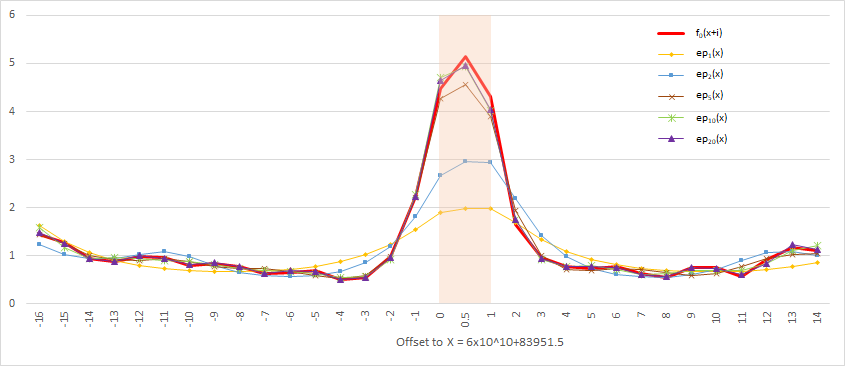
\includegraphics[width=\linewidth]{euler_product_approximation.png}
  \caption{Improving approximation of ep$_n(x)$ w.r.t. $|f_0(x+iy)|$ as n is increased, where ep$_n(x)$=eulerprod$(x,p_n)$, shown near $X=6 \times 10^{10} + 83951.5$, which was chosen as a barrier location.}
	\label{euler}
\end{figure}

